\documentclass[dvipsnames]{article}%
\usepackage[T1]{fontenc}%
\usepackage[utf8]{inputenc}%
\usepackage{lmodern}%
\usepackage{textcomp}%
\usepackage{lastpage}%
\usepackage{graphicx}%
\usepackage{placeins}%
\usepackage{calc}%
\usepackage{tikz}%
\usepackage{xcolor}%
\usepackage{fancyhdr}%
\usepackage{subfig}%
\usepackage{geometry}%
\usepackage{booktabs}%
%
\usepackage[utf8]{inputenc}%
\usepackage[brazil]{babel}%
\setlength{\headsep}{3cm}%
\setlength{\footskip}{1cm}%
\geometry{top=4cm}%
\fancyhead[L]{
\includegraphics[width=0.1\paperwidth]{report_images/logo_2.png}}%
\fancyhead[R]{Relatóriio Termográfico}%
\fancyfoot[C]{GreTA®, Versão Beta - 2025 \quad Desenvolvido por Aisol}%
\usetikzlibrary{calc}%
%
\begin{document}%
\normalsize%
\thispagestyle{empty}%

\begin{tikzpicture}[overlay,remember picture]

% Rectangles
\shade[
left color=lightgray, 
right color=NavyBlue!40,
transform canvas ={rotate around ={45:($(current page.north west)+(0,-6)$)}}] 
($(current page.north west)+(0,-6)$) rectangle ++(9,1.5);

\shade[
left color=lightgray,
right color=lightgray!50,
rounded corners=0.75cm,
transform canvas ={rotate around ={45:($(current page.north west)+(.5,-10)$)}}]
($(current page.north west)+(0.5,-10)$) rectangle ++(15,1.5);

\shade[
left color=lightgray,
rounded corners=0.3cm,
transform canvas ={rotate around ={45:($(current page.north west)+(.5,-10)$)}}] ($(current page.north west)+(1.5,-9.55)$) rectangle ++(7,.6);

\shade[
left color=lightgray!80,
right color=blue!60,
rounded corners=0.4cm,
transform canvas ={rotate around ={45:($(current page.north)+(-1.5,-3)$)}}]
($(current page.north)+(-1.5,-3)$) rectangle ++(9,0.8);

\shade[
left color=RoyalBlue!80,
right color=blue!80,
rounded corners=0.9cm,
transform canvas ={rotate around ={45:($(current page.north)+(-3,-8)$)}}] ($(current page.north)+(-3,-8)$) rectangle ++(15,1.8);

\shade[
left color=lightgray,
right color=RoyalBlue,
rounded corners=0.9cm,
transform canvas ={rotate around ={45:($(current page.north west)+(4,-15.5)$)}}]
($(current page.north west)+(4,-15.5)$) rectangle ++(30,1.8);

\shade[
left color=RoyalBlue,
right color=Emerald,
rounded corners=0.75cm,
transform canvas ={rotate around ={45:($(current page.north west)+(13,-10)$)}}]
($(current page.north west)+(13,-10)$) rectangle ++(15,1.5);

\shade[
left color=lightgray,
rounded corners=0.3cm,
transform canvas ={rotate around ={45:($(current page.north west)+(18,-8)$)}}]
($(current page.north west)+(18,-8)$) rectangle ++(15,0.6);

\shade[
left color=lightgray,
rounded corners=0.4cm,
transform canvas ={rotate around ={45:($(current page.north west)+(19,-5.65)$)}}]
($(current page.north west)+(19,-5.65)$) rectangle ++(15,0.8);

\shade[
left color=RoyalBlue,
right color=red!80,
rounded corners=0.6cm,
transform canvas ={rotate around ={45:($(current page.north west)+(20,-9)$)}}] 
($(current page.north west)+(20,-9)$) rectangle ++(14,1.2);

% Year
\draw[ultra thick,gray]
($(current page.center)+(5,2)$) -- ++(0,-3cm) 
node[
midway,
left=0.25cm,
text width=5cm,
align=right,
black!75
]
{
{\fontsize{25}{30} \selectfont \bf Área \\[10pt] 1}
} 
node[
midway,
right=0.25cm,
text width=6cm,
align=left,
RoyalBlue]
{
{\fontsize{72}{86.4} \selectfont 2025}
};

% Title
\node[align=center] at ($(current page.center)+(0,-5)$) 
{
{\fontsize{60}{72} \selectfont {{Relatório Termográfico}}} \\[1cm]
{\fontsize{16}{19.2} \selectfont \textcolor{RoyalBlue}{ \bf Relatório Físico}}\\[3pt]};
\node[align=center] at ($(current page.center)+(0,-9.5)$) 
{ Desenvolvido por:};
\node[align=center] at ($(current page.center)+(0,-11)$) 
{
\includegraphics[width=0.4\paperwidth]{report_images/logo_2.png}};


\end{tikzpicture}%
\newpage%
\thispagestyle{empty}%
\vspace*{0.4cm}%
\rule{\linewidth}{0.5pt}%
\begin{center}%
{\large\bfseries Relatório de Inspeção por Imagem Térmica.  }%
\vspace*{0.5cm}%
\textbf{Responsável Técnico:} ANONIMIZADO, Engineer.  %
\textbf{CREA:} 12345678  %
\textbf{Date:} March 2025%
\textbf{Localização:} Campo Grande, MS. Brasil.  %
\textbf{Endereço:} Rua Manoel Inácio de Souza, n. 24, C.E.P : 79.020-220  %
\textbf{Software:} GreTA® - Georeferenced Thermographic Analysis System, Versão Beta.  %
\textbf{Versão:} Versão ANONIMIZADA  %
\end{center}%
\vspace*{0.4cm}%
\rule{\linewidth}{0.5pt}%
\vfill%
\noindent\textbf{Copyright © 2025 Aisol Soluções em Inteligência Artificial.  }%
Todos os direitos reservados. Nenhuma parte desta publicação pode ser reproduzida, distribuída ou transmitida sem autorização prévia.  %
\vspace*{0.2cm}%
\noindent\textbf{ISBN:} xxxxxxxx.  %
\textbf{Location:}%
Campo Grande, MS. Brasil.  %
Rua Manoel Inácio de Souza, n. 24.  %
C.E.P : 79.020{-}220.  %
\textbf{Copyrights:}%
Aisol, 2023.  %
\textbf{Release:}%
VERSAO ANONIMIZADA.  %
\textbf{Company:}%
Aisol Soluções em Inteligência Artificial em parceria com PVX Engenharia.  %
\newpage%
\tableofcontents%
\newpage%
\newpage%
\begin{abstract}%
As inspeções termográficas tornaram-se uma ferramenta essencial para avaliar o desempenho e a confiabilidade de usinas solares. Este estudo foca na detecção e análise de \textbf{pontos quentes (hotspots), diodos de bypass queimados e painéis ou strings inativos}, indicadores críticos de ineficiências operacionais. \textbf{Hotspots} aparecem como regiões de alta temperatura localizadas nos painéis solares, frequentemente causadas por sombreamento, acúmulo de sujeira ou células fotovoltaicas defeituosas, podendo levar à degradação do desempenho e danos a longo prazo. \textbf{Diodos de bypass queimados} interrompem o fluxo elétrico esperado, causando o superaquecimento de fileiras inteiras de células (\textbf{hot lines}), o que pode reduzir significativamente a eficiência do sistema. Além disso, \textbf{painéis ou strings inativos} — identificados como regiões mais frias do que o esperado nas imagens térmicas — indicam possíveis falhas em inversores, desconexões ou problemas elétricos. A detecção precoce e a implementação de ações corretivas direcionadas podem otimizar a geração de energia, prolongar a vida útil do sistema e prevenir falhas onerosas.%
\end{abstract}%
\pagestyle{fancy}%
\section{Introduction}%
A termografia, utilizando tecnologia infravermelha, é uma ferramenta fundamental para identificar discrepâncias térmicas em instalações solares. Este relatório emprega metodologias termográficas avançadas para detectar e localizar \textbf{pontos quentes (hotspots)} em painéis solares e rastreadores. Esses hotspots, caracterizados por regiões de temperatura elevada, geralmente indicam anomalias operacionais ou ineficiências materiais na infraestrutura. 

A primeira seção do relatório, \textbf{Dados do Cliente}, apresenta um conjunto de dados que inclui identificadores específicos do cliente e especificações dos equipamentos. Em seguida, a \textbf{Visão Geral da Área} oferece uma representação espacial do local da instalação. Utilizando coordenadas geoespaciais, esta seção fornece um layout escalado dos painéis solares e rastreadores, estabelecendo uma matriz de referência. 

%
\section{Dados do Cliente}%
Anonimizado%
\section{Visão Geral da Área}%
 Nesta seção, apresentamos uma visão abrangente da área inspecionada. A \textbf{Figura 1} exibe a \textbf{ortofoto} montada a partir de todas as imagens capturadas da região. A \textbf{Figura 2} apresenta uma representação esquemática da área, destacando as localizações dos rastreadores e dos hotspots detectados. A numeração dos rastreadores segue o padrão: da esquerda para a direita (de oeste para leste) e de cima para baixo (de norte para sul).%
\FloatBarrier%


\begin{figure}[h!]%
\centering%
\includegraphics[width=0.6\linewidth]{report_images/ortho.png}%
\caption{Ortofoto}%
\end{figure}

%
\FloatBarrier%


\begin{figure}[h!]%
\centering%
\includegraphics[width=0.6\linewidth]{report_images/layer_img.pdf}%
\caption{Máscara dos Painéis}%
\end{figure}

%
\FloatBarrier%


\begin{table}[h!]%
\caption{Resumo dos Defeitos Identificados}%
\centering%
\begin{tabular}{lcl}%
\toprule%
Tipo de Problema&Local do Painel&Coordenadas\\%
\midrule%
Pontos Quentes (Hot Spots)&2{-}70&ANONIMIZADO\\%
Pontos Quentes (Hot Spots)&2{-}70&ANONIMIZADO\\%
Pontos Quentes (Hot Spots)&2{-}114&ANONIMIZADO\\%
Pontos Quentes (Hot Spots)&2{-}114&ANONIMIZADO\\%
Pontos Quentes (Hot Spots)&2{-}118&ANONIMIZADO\\%
Pontos Quentes (Hot Spots)&2{-}118&ANONIMIZADO\\%
Pontos Quentes (Hot Spots)&4{-}109&ANONIMIZADO\\%
Pontos Quentes (Hot Spots)&4{-}109&ANONIMIZADO\\%
Pontos Quentes (Hot Spots)&4{-}122&ANONIMIZADO\\%
Pontos Quentes (Hot Spots)&4{-}122&ANONIMIZADO\\%
Pontos Quentes (Hot Spots)&5{-}96&ANONIMIZADO\\%
Pontos Quentes (Hot Spots)&5{-}97&ANONIMIZADO\\%
Pontos Quentes (Hot Spots)&5{-}97&ANONIMIZADO\\%
Pontos Quentes (Hot Spots)&5{-}98&ANONIMIZADO\\%
Pontos Quentes (Hot Spots)&5{-}104&ANONIMIZADO\\%
Pontos Quentes (Hot Spots)&5{-}104&ANONIMIZADO\\%
Pontos Quentes (Hot Spots)&5{-}114&ANONIMIZADO\\%
Pontos Quentes (Hot Spots)&5{-}114&ANONIMIZADO\\%
Pontos Quentes (Hot Spots)&5{-}115&ANONIMIZADO\\%
Pontos Quentes (Hot Spots)&6{-}22&ANONIMIZADO\\%
Pontos Quentes (Hot Spots)&6{-}68&ANONIMIZADO\\%
Pontos Quentes (Hot Spots)&6{-}68&ANONIMIZADO\\%
Pontos Quentes (Hot Spots)&6{-}68&ANONIMIZADO\\%
Pontos Quentes (Hot Spots)&6{-}78&ANONIMIZADO\\%
Pontos Quentes (Hot Spots)&6{-}78&ANONIMIZADO\\%
Pontos Quentes (Hot Spots)&6{-}105&ANONIMIZADO\\%
Pontos Quentes (Hot Spots)&6{-}105&ANONIMIZADO\\%
Pontos Quentes (Hot Spots)&6{-}106&ANONIMIZADO\\%
Pontos Quentes (Hot Spots)&6{-}106&ANONIMIZADO\\%
Pontos Quentes (Hot Spots)&7{-}15&ANONIMIZADO\\%
Pontos Quentes (Hot Spots)&7{-}15&ANONIMIZADO\\%
Pontos Quentes (Hot Spots)&7{-}63&ANONIMIZADO\\%
Pontos Quentes (Hot Spots)&7{-}63&ANONIMIZADO\\%
Pontos Quentes (Hot Spots)&7{-}97&ANONIMIZADO\\%
Pontos Quentes (Hot Spots)&7{-}97&ANONIMIZADO\\%
\bottomrule%
\end{tabular}%
\end{table}

%
\FloatBarrier%


\begin{table}[h!]%
\caption{Resumo dos Defeitos Identificados (cont.)}%
\centering%
\begin{tabular}{lcl}%
\toprule%
Tipo de Problema&Local do Painel&Coordenadas\\%
\midrule%
Pontos Quentes (Hot Spots)&7{-}120&ANONIMIZADO\\%
Pontos Quentes (Hot Spots)&7{-}120&ANONIMIZADO\\%
Pontos Quentes (Hot Spots)&8{-}35&ANONIMIZADO\\%
Pontos Quentes (Hot Spots)&8{-}35&ANONIMIZADO\\%
Pontos Quentes (Hot Spots)&8{-}35&ANONIMIZADO\\%
Pontos Quentes (Hot Spots)&8{-}36&ANONIMIZADO\\%
Pontos Quentes (Hot Spots)&8{-}36&ANONIMIZADO\\%
Pontos Quentes (Hot Spots)&8{-}37&ANONIMIZADO\\%
Pontos Quentes (Hot Spots)&8{-}37&ANONIMIZADO\\%
Pontos Quentes (Hot Spots)&8{-}117&ANONIMIZADO\\%
Pontos Quentes (Hot Spots)&8{-}117&ANONIMIZADO\\%
Pontos Quentes (Hot Spots)&8{-}122&ANONIMIZADO\\%
Pontos Quentes (Hot Spots)&8{-}122&ANONIMIZADO\\%
Pontos Quentes (Hot Spots)&9{-}43&ANONIMIZADO\\%
Pontos Quentes (Hot Spots)&9{-}43&ANONIMIZADO\\%
Pontos Quentes (Hot Spots)&9{-}92&ANONIMIZADO\\%
Pontos Quentes (Hot Spots)&9{-}92&ANONIMIZADO\\%
Pontos Quentes (Hot Spots)&10{-}53&ANONIMIZADO\\%
Pontos Quentes (Hot Spots)&10{-}53&ANONIMIZADO\\%
Pontos Quentes (Hot Spots)&11{-}61&ANONIMIZADO\\%
Pontos Quentes (Hot Spots)&11{-}61&ANONIMIZADO\\%
Pontos Quentes (Hot Spots)&12{-}22&ANONIMIZADO\\%
Pontos Quentes (Hot Spots)&12{-}56&ANONIMIZADO\\%
Pontos Quentes (Hot Spots)&12{-}56&ANONIMIZADO\\%
Pontos Quentes (Hot Spots)&12{-}56&ANONIMIZADO\\%
Pontos Quentes (Hot Spots)&12{-}61&ANONIMIZADO\\%
Pontos Quentes (Hot Spots)&12{-}61&ANONIMIZADO\\%
Pontos Quentes (Hot Spots)&13{-}10&ANONIMIZADO\\%
Pontos Quentes (Hot Spots)&13{-}10&ANONIMIZADO\\%
Pontos Quentes (Hot Spots)&13{-}16&ANONIMIZADO\\%
Pontos Quentes (Hot Spots)&13{-}16&ANONIMIZADO\\%
Pontos Quentes (Hot Spots)&13{-}18&ANONIMIZADO\\%
Pontos Quentes (Hot Spots)&13{-}18&ANONIMIZADO\\%
Pontos Quentes (Hot Spots)&13{-}18&ANONIMIZADO\\%
Pontos Quentes (Hot Spots)&13{-}55&ANONIMIZADO\\%
\bottomrule%
\end{tabular}%
\end{table}

%
\FloatBarrier%


\begin{table}[h!]%
\caption{Resumo dos Defeitos Identificados (cont.)}%
\centering%
\begin{tabular}{lcl}%
\toprule%
Tipo de Problema&Local do Painel&Coordenadas\\%
\midrule%
Pontos Quentes (Hot Spots)&13{-}56&ANONIMIZADO\\%
Pontos Quentes (Hot Spots)&13{-}60&ANONIMIZADO\\%
Pontos Quentes (Hot Spots)&13{-}60&ANONIMIZADO\\%
Pontos Quentes (Hot Spots)&13{-}62&ANONIMIZADO\\%
Pontos Quentes (Hot Spots)&13{-}62&ANONIMIZADO\\%
\bottomrule%
\end{tabular}%
\end{table}

%
\FloatBarrier%
\newpage%
\section{Pontos Quentes (Hot Spots)}%
Foram detectados pontos quentes nas placas abaixo.\newline%
%
\subsubsection{Painel 2-70}%


\begin{figure}[h!]%
\centering%
\subfloat[Recorte do Painel em Análise]{\includegraphics[width=0.31\linewidth]{report_images/hotspots_(2-70)_layer.pdf}}%
\hfill%
\subfloat[Localização do Problema]{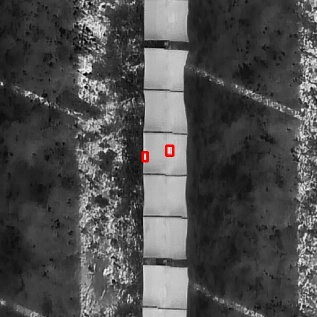
\includegraphics[width=0.31\linewidth]{report_images/hotspots_(2-70)_cropped.jpg}}%
\hfill%
\subfloat[Imagem Original do Drone]{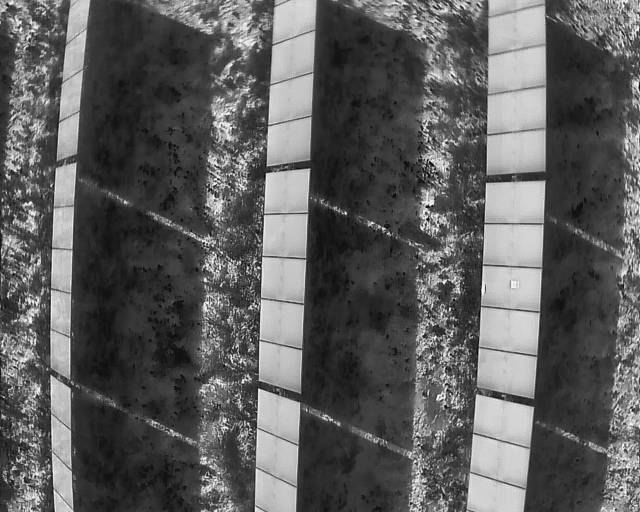
\includegraphics[width=0.31\linewidth]{report_images/hotspots_(2-70).jpg}}%
\caption{Imagens do Painel n. 70 da coluna n. 2.}%
\end{figure}

%
\FloatBarrier%
No painel 2{-}70, há sinais de pontos quentes conforme as figuras acima.\newline%
%
\subsubsection{Painel 2-114}%


\begin{figure}[h!]%
\centering%
\subfloat[Recorte do Painel em Análise]{\includegraphics[width=0.31\linewidth]{report_images/hotspots_(2-114)_layer.pdf}}%
\hfill%
\subfloat[Localização do Problema]{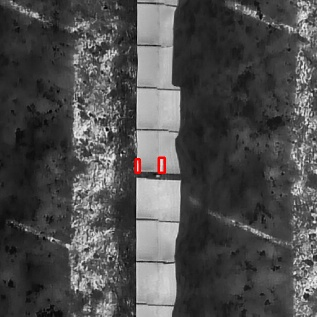
\includegraphics[width=0.31\linewidth]{report_images/hotspots_(2-114)_cropped.jpg}}%
\hfill%
\subfloat[Imagem Original do Drone]{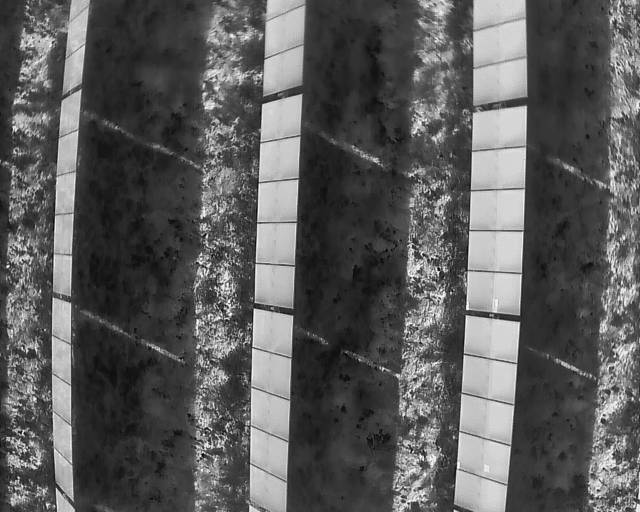
\includegraphics[width=0.31\linewidth]{report_images/hotspots_(2-114).jpg}}%
\caption{Imagens do Painel n. 114 da coluna n. 2.}%
\end{figure}

%
\FloatBarrier%
No painel 2{-}114, há sinais de pontos quentes conforme as figuras acima.\newline%
%
\subsubsection{Painel 2-118}%


\begin{figure}[h!]%
\centering%
\subfloat[Recorte do Painel em Análise]{\includegraphics[width=0.31\linewidth]{report_images/hotspots_(2-118)_layer.pdf}}%
\hfill%
\subfloat[Localização do Problema]{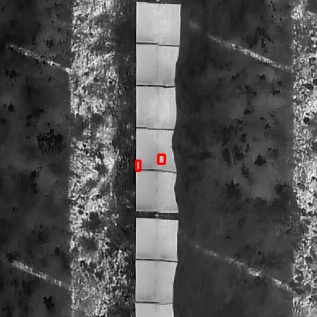
\includegraphics[width=0.31\linewidth]{report_images/hotspots_(2-118)_cropped.jpg}}%
\hfill%
\subfloat[Imagem Original do Drone]{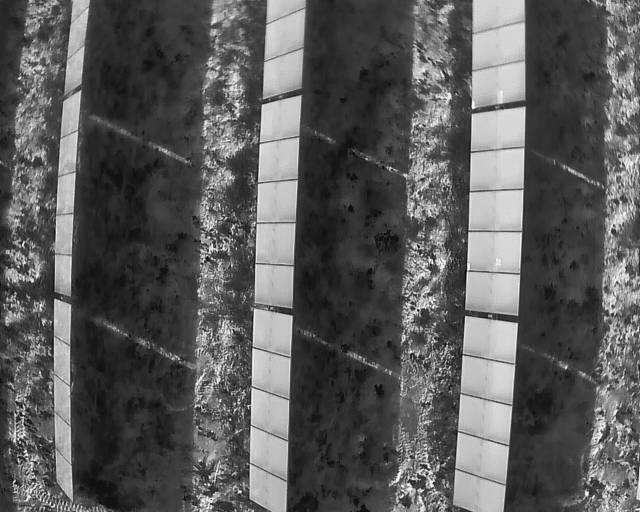
\includegraphics[width=0.31\linewidth]{report_images/hotspots_(2-118).jpg}}%
\caption{Imagens do Painel n. 118 da coluna n. 2.}%
\end{figure}

%
\FloatBarrier%
No painel 2{-}118, há sinais de pontos quentes conforme as figuras acima.\newline%
%
\subsubsection{Painel 4-109}%


\begin{figure}[h!]%
\centering%
\subfloat[Recorte do Painel em Análise]{\includegraphics[width=0.31\linewidth]{report_images/hotspots_(4-109)_layer.pdf}}%
\hfill%
\subfloat[Localização do Problema]{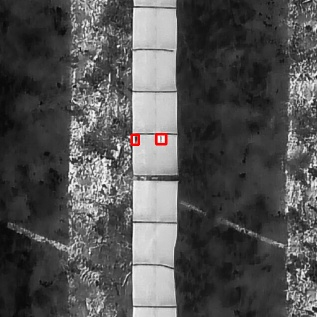
\includegraphics[width=0.31\linewidth]{report_images/hotspots_(4-109)_cropped.jpg}}%
\hfill%
\subfloat[Imagem Original do Drone]{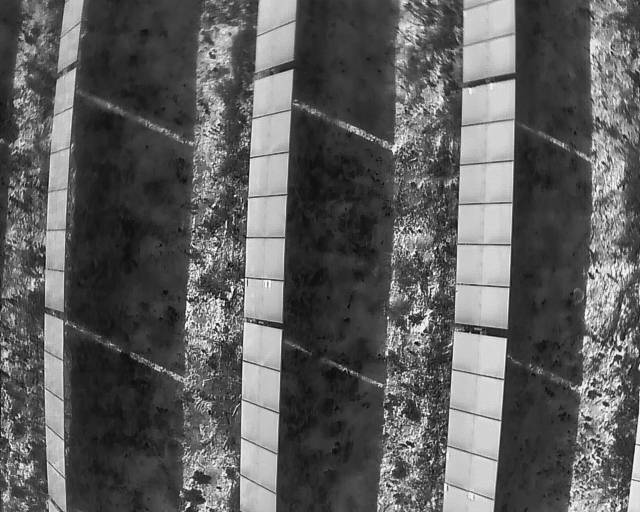
\includegraphics[width=0.31\linewidth]{report_images/hotspots_(4-109).jpg}}%
\caption{Imagens do Painel n. 109 da coluna n. 4.}%
\end{figure}

%
\FloatBarrier%
No painel 4{-}109, há sinais de pontos quentes conforme as figuras acima.\newline%
%
\subsubsection{Painel 4-122}%


\begin{figure}[h!]%
\centering%
\subfloat[Recorte do Painel em Análise]{\includegraphics[width=0.31\linewidth]{report_images/hotspots_(4-122)_layer.pdf}}%
\hfill%
\subfloat[Localização do Problema]{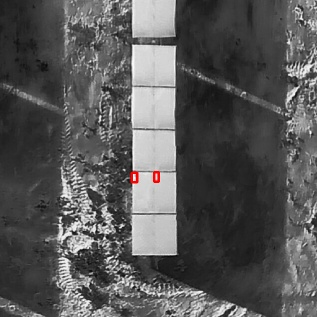
\includegraphics[width=0.31\linewidth]{report_images/hotspots_(4-122)_cropped.jpg}}%
\hfill%
\subfloat[Imagem Original do Drone]{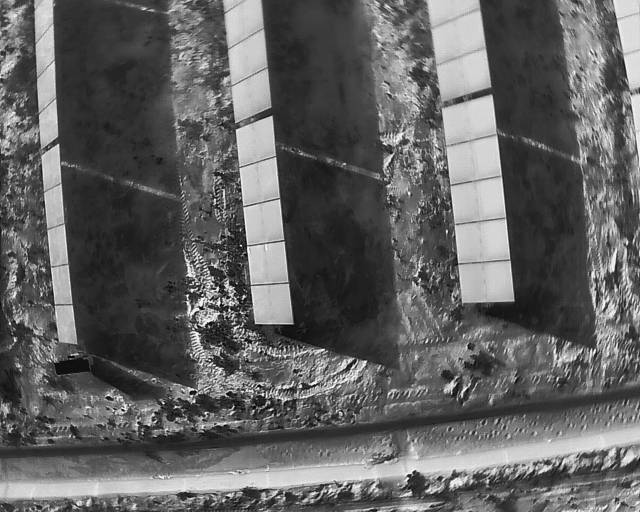
\includegraphics[width=0.31\linewidth]{report_images/hotspots_(4-122).jpg}}%
\caption{Imagens do Painel n. 122 da coluna n. 4.}%
\end{figure}

%
\FloatBarrier%
No painel 4{-}122, há sinais de pontos quentes conforme as figuras acima.\newline%
%
\subsubsection{Painel 5-96}%


\begin{figure}[h!]%
\centering%
\subfloat[Recorte do Painel em Análise]{\includegraphics[width=0.31\linewidth]{report_images/hotspots_(5-96)_layer.pdf}}%
\hfill%
\subfloat[Localização do Problema]{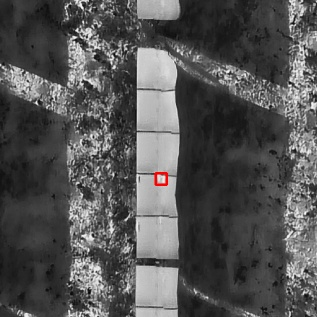
\includegraphics[width=0.31\linewidth]{report_images/hotspots_(5-96)_cropped.jpg}}%
\hfill%
\subfloat[Imagem Original do Drone]{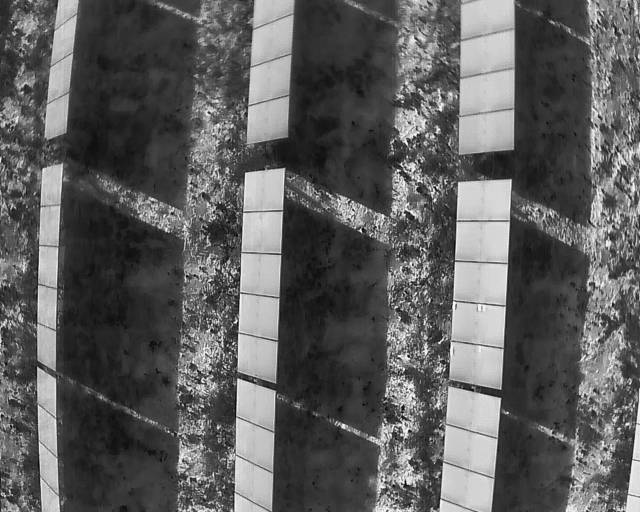
\includegraphics[width=0.31\linewidth]{report_images/hotspots_(5-96).jpg}}%
\caption{Imagens do Painel n. 96 da coluna n. 5.}%
\end{figure}

%
\FloatBarrier%
No painel 5{-}96, há sinais de pontos quentes conforme as figuras acima.\newline%
%
\subsubsection{Painel 5-97}%


\begin{figure}[h!]%
\centering%
\subfloat[Recorte do Painel em Análise]{\includegraphics[width=0.31\linewidth]{report_images/hotspots_(5-97)_layer.pdf}}%
\hfill%
\subfloat[Localização do Problema]{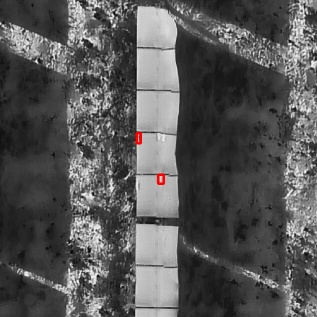
\includegraphics[width=0.31\linewidth]{report_images/hotspots_(5-97)_cropped.jpg}}%
\hfill%
\subfloat[Imagem Original do Drone]{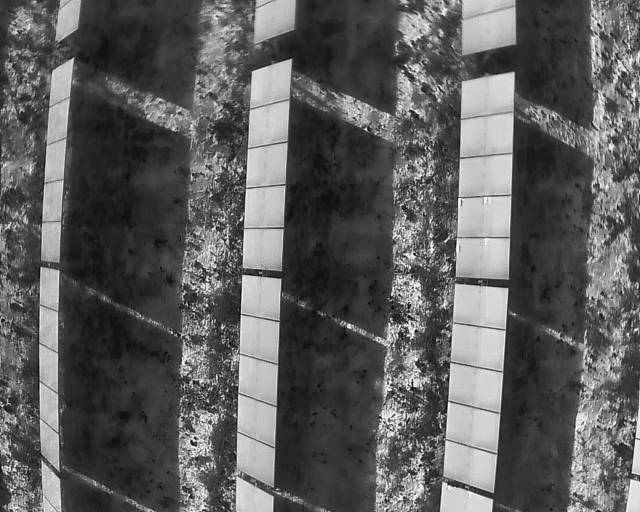
\includegraphics[width=0.31\linewidth]{report_images/hotspots_(5-97).jpg}}%
\caption{Imagens do Painel n. 97 da coluna n. 5.}%
\end{figure}

%
\FloatBarrier%
No painel 5{-}97, há sinais de pontos quentes conforme as figuras acima.\newline%
%
\subsubsection{Painel 5-98}%


\begin{figure}[h!]%
\centering%
\subfloat[Recorte do Painel em Análise]{\includegraphics[width=0.31\linewidth]{report_images/hotspots_(5-98)_layer.pdf}}%
\hfill%
\subfloat[Localização do Problema]{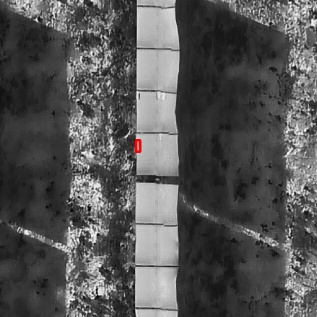
\includegraphics[width=0.31\linewidth]{report_images/hotspots_(5-98)_cropped.jpg}}%
\hfill%
\subfloat[Imagem Original do Drone]{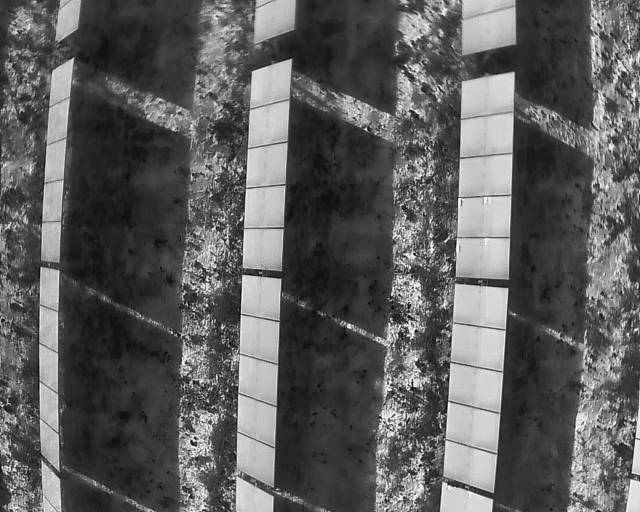
\includegraphics[width=0.31\linewidth]{report_images/hotspots_(5-98).jpg}}%
\caption{Imagens do Painel n. 98 da coluna n. 5.}%
\end{figure}

%
\FloatBarrier%
No painel 5{-}98, há sinais de pontos quentes conforme as figuras acima.\newline%
%
\subsubsection{Painel 5-104}%


\begin{figure}[h!]%
\centering%
\subfloat[Recorte do Painel em Análise]{\includegraphics[width=0.31\linewidth]{report_images/hotspots_(5-104)_layer.pdf}}%
\hfill%
\subfloat[Localização do Problema]{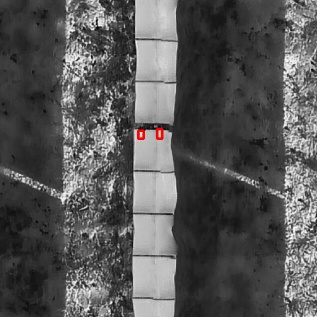
\includegraphics[width=0.31\linewidth]{report_images/hotspots_(5-104)_cropped.jpg}}%
\hfill%
\subfloat[Imagem Original do Drone]{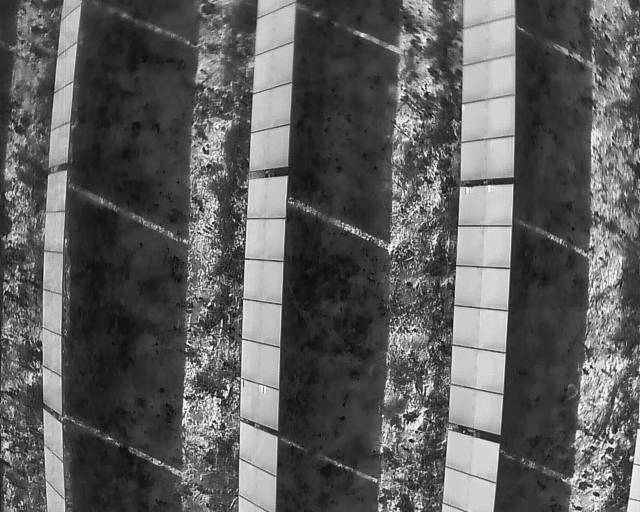
\includegraphics[width=0.31\linewidth]{report_images/hotspots_(5-104).jpg}}%
\caption{Imagens do Painel n. 104 da coluna n. 5.}%
\end{figure}

%
\FloatBarrier%
No painel 5{-}104, há sinais de pontos quentes conforme as figuras acima.\newline%
%
\subsubsection{Painel 5-114}%


\begin{figure}[h!]%
\centering%
\subfloat[Recorte do Painel em Análise]{\includegraphics[width=0.31\linewidth]{report_images/hotspots_(5-114)_layer.pdf}}%
\hfill%
\subfloat[Localização do Problema]{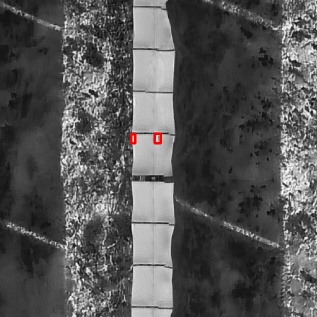
\includegraphics[width=0.31\linewidth]{report_images/hotspots_(5-114)_cropped.jpg}}%
\hfill%
\subfloat[Imagem Original do Drone]{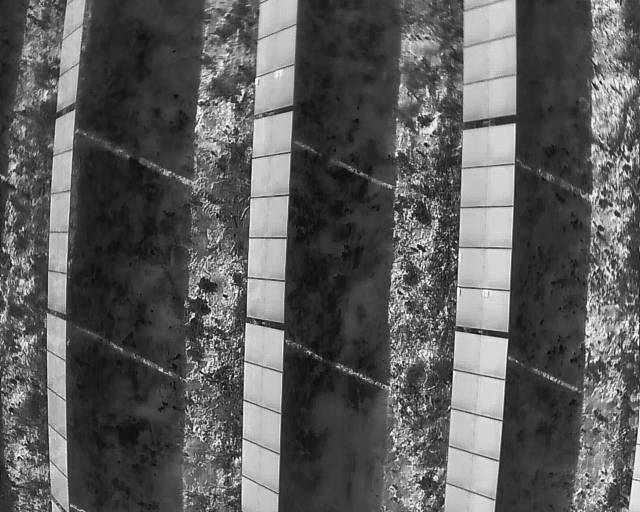
\includegraphics[width=0.31\linewidth]{report_images/hotspots_(5-114).jpg}}%
\caption{Imagens do Painel n. 114 da coluna n. 5.}%
\end{figure}

%
\FloatBarrier%
No painel 5{-}114, há sinais de pontos quentes conforme as figuras acima.\newline%
%
\subsubsection{Painel 5-115}%


\begin{figure}[h!]%
\centering%
\subfloat[Recorte do Painel em Análise]{\includegraphics[width=0.31\linewidth]{report_images/hotspots_(5-115)_layer.pdf}}%
\hfill%
\subfloat[Localização do Problema]{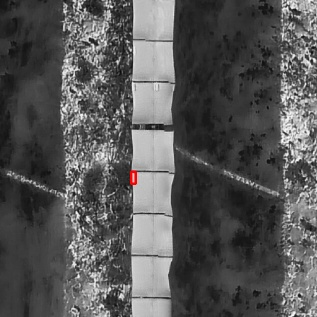
\includegraphics[width=0.31\linewidth]{report_images/hotspots_(5-115)_cropped.jpg}}%
\hfill%
\subfloat[Imagem Original do Drone]{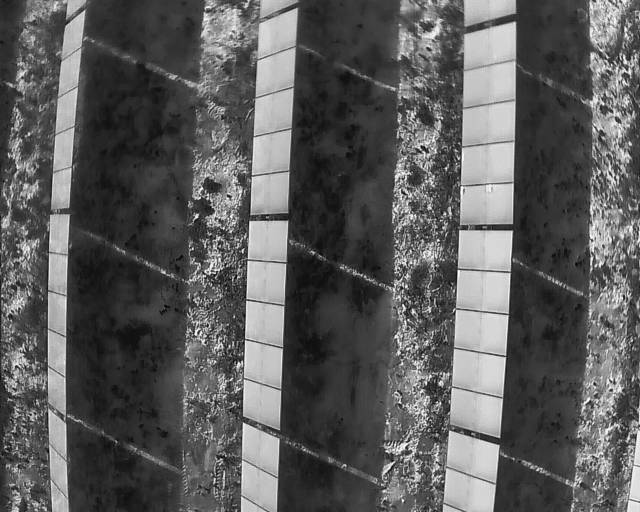
\includegraphics[width=0.31\linewidth]{report_images/hotspots_(5-115).jpg}}%
\caption{Imagens do Painel n. 115 da coluna n. 5.}%
\end{figure}

%
\FloatBarrier%
No painel 5{-}115, há sinais de pontos quentes conforme as figuras acima.\newline%
%
\subsubsection{Painel 6-22}%


\begin{figure}[h!]%
\centering%
\subfloat[Recorte do Painel em Análise]{\includegraphics[width=0.31\linewidth]{report_images/hotspots_(6-22)_layer.pdf}}%
\hfill%
\subfloat[Localização do Problema]{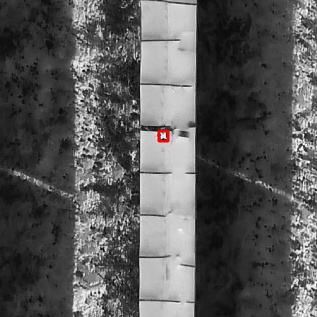
\includegraphics[width=0.31\linewidth]{report_images/hotspots_(6-22)_cropped.jpg}}%
\hfill%
\subfloat[Imagem Original do Drone]{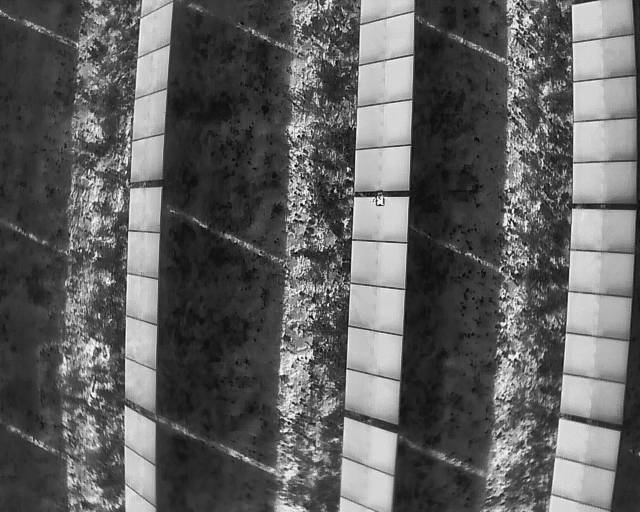
\includegraphics[width=0.31\linewidth]{report_images/hotspots_(6-22).jpg}}%
\caption{Imagens do Painel n. 22 da coluna n. 6.}%
\end{figure}

%
\FloatBarrier%
No painel 6{-}22, há sinais de pontos quentes conforme as figuras acima.\newline%
%
\subsubsection{Painel 6-68}%


\begin{figure}[h!]%
\centering%
\subfloat[Recorte do Painel em Análise]{\includegraphics[width=0.31\linewidth]{report_images/hotspots_(6-68)_layer.pdf}}%
\hfill%
\subfloat[Localização do Problema]{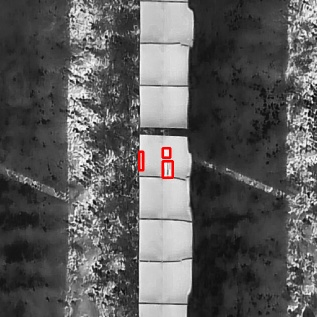
\includegraphics[width=0.31\linewidth]{report_images/hotspots_(6-68)_cropped.jpg}}%
\hfill%
\subfloat[Imagem Original do Drone]{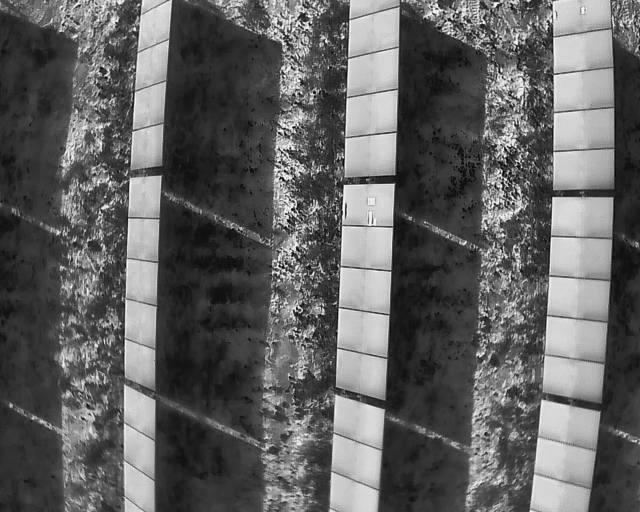
\includegraphics[width=0.31\linewidth]{report_images/hotspots_(6-68).jpg}}%
\caption{Imagens do Painel n. 68 da coluna n. 6.}%
\end{figure}

%
\FloatBarrier%
No painel 6{-}68, há sinais de pontos quentes conforme as figuras acima.\newline%
%
\subsubsection{Painel 6-78}%


\begin{figure}[h!]%
\centering%
\subfloat[Recorte do Painel em Análise]{\includegraphics[width=0.31\linewidth]{report_images/hotspots_(6-78)_layer.pdf}}%
\hfill%
\subfloat[Localização do Problema]{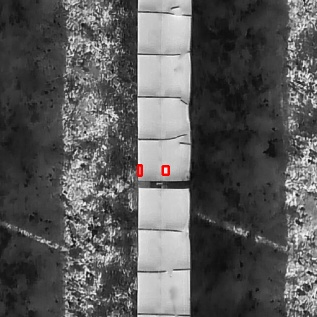
\includegraphics[width=0.31\linewidth]{report_images/hotspots_(6-78)_cropped.jpg}}%
\hfill%
\subfloat[Imagem Original do Drone]{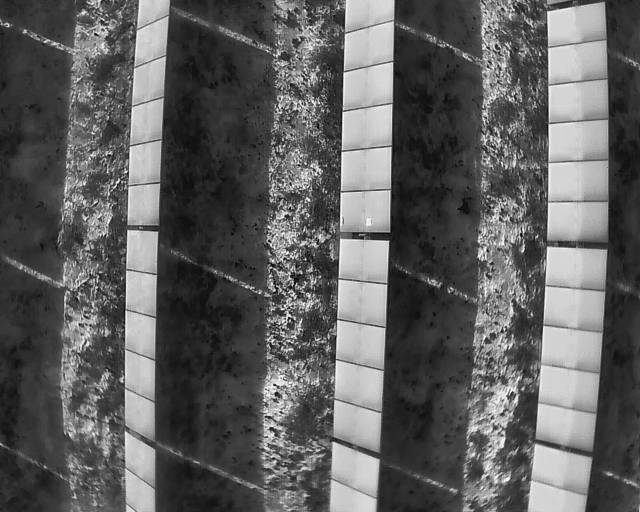
\includegraphics[width=0.31\linewidth]{report_images/hotspots_(6-78).jpg}}%
\caption{Imagens do Painel n. 78 da coluna n. 6.}%
\end{figure}

%
\FloatBarrier%
No painel 6{-}78, há sinais de pontos quentes conforme as figuras acima.\newline%
%
\subsubsection{Painel 6-105}%


\begin{figure}[h!]%
\centering%
\subfloat[Recorte do Painel em Análise]{\includegraphics[width=0.31\linewidth]{report_images/hotspots_(6-105)_layer.pdf}}%
\hfill%
\subfloat[Localização do Problema]{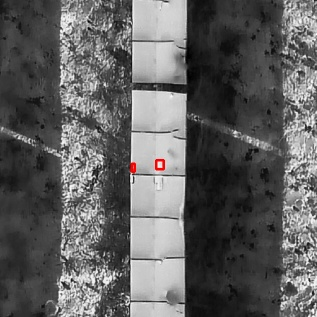
\includegraphics[width=0.31\linewidth]{report_images/hotspots_(6-105)_cropped.jpg}}%
\hfill%
\subfloat[Imagem Original do Drone]{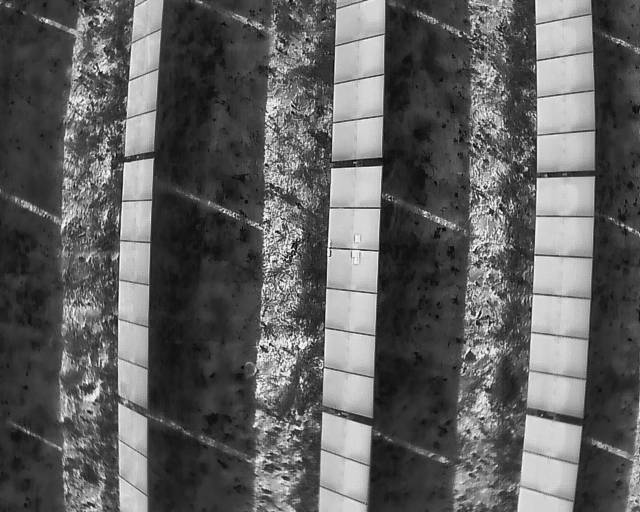
\includegraphics[width=0.31\linewidth]{report_images/hotspots_(6-105).jpg}}%
\caption{Imagens do Painel n. 105 da coluna n. 6.}%
\end{figure}

%
\FloatBarrier%
No painel 6{-}105, há sinais de pontos quentes conforme as figuras acima.\newline%
%
\subsubsection{Painel 6-106}%


\begin{figure}[h!]%
\centering%
\subfloat[Recorte do Painel em Análise]{\includegraphics[width=0.31\linewidth]{report_images/hotspots_(6-106)_layer.pdf}}%
\hfill%
\subfloat[Localização do Problema]{\includegraphics[width=0.31\linewidth]{report_images/hotspots_(6-106)_cropped.jpg}}%
\hfill%
\subfloat[Imagem Original do Drone]{\includegraphics[width=0.31\linewidth]{report_images/hotspots_(6-106).jpg}}%
\caption{Imagens do Painel n. 106 da coluna n. 6.}%
\end{figure}

%
\FloatBarrier%
No painel 6{-}106, há sinais de pontos quentes conforme as figuras acima.\newline%
%
\subsubsection{Painel 7-15}%


\begin{figure}[h!]%
\centering%
\subfloat[Recorte do Painel em Análise]{\includegraphics[width=0.31\linewidth]{report_images/hotspots_(7-15)_layer.pdf}}%
\hfill%
\subfloat[Localização do Problema]{\includegraphics[width=0.31\linewidth]{report_images/hotspots_(7-15)_cropped.jpg}}%
\hfill%
\subfloat[Imagem Original do Drone]{\includegraphics[width=0.31\linewidth]{report_images/hotspots_(7-15).jpg}}%
\caption{Imagens do Painel n. 15 da coluna n. 7.}%
\end{figure}

%
\FloatBarrier%
No painel 7{-}15, há sinais de pontos quentes conforme as figuras acima.\newline%
%
\subsubsection{Painel 7-63}%


\begin{figure}[h!]%
\centering%
\subfloat[Recorte do Painel em Análise]{\includegraphics[width=0.31\linewidth]{report_images/hotspots_(7-63)_layer.pdf}}%
\hfill%
\subfloat[Localização do Problema]{\includegraphics[width=0.31\linewidth]{report_images/hotspots_(7-63)_cropped.jpg}}%
\hfill%
\subfloat[Imagem Original do Drone]{\includegraphics[width=0.31\linewidth]{report_images/hotspots_(7-63).jpg}}%
\caption{Imagens do Painel n. 63 da coluna n. 7.}%
\end{figure}

%
\FloatBarrier%
No painel 7{-}63, há sinais de pontos quentes conforme as figuras acima.\newline%
%
\subsubsection{Painel 7-97}%


\begin{figure}[h!]%
\centering%
\subfloat[Recorte do Painel em Análise]{\includegraphics[width=0.31\linewidth]{report_images/hotspots_(7-97)_layer.pdf}}%
\hfill%
\subfloat[Localização do Problema]{\includegraphics[width=0.31\linewidth]{report_images/hotspots_(7-97)_cropped.jpg}}%
\hfill%
\subfloat[Imagem Original do Drone]{\includegraphics[width=0.31\linewidth]{report_images/hotspots_(7-97).jpg}}%
\caption{Imagens do Painel n. 97 da coluna n. 7.}%
\end{figure}

%
\FloatBarrier%
No painel 7{-}97, há sinais de pontos quentes conforme as figuras acima.\newline%
%
\subsubsection{Painel 7-120}%


\begin{figure}[h!]%
\centering%
\subfloat[Recorte do Painel em Análise]{\includegraphics[width=0.31\linewidth]{report_images/hotspots_(7-120)_layer.pdf}}%
\hfill%
\subfloat[Localização do Problema]{\includegraphics[width=0.31\linewidth]{report_images/hotspots_(7-120)_cropped.jpg}}%
\hfill%
\subfloat[Imagem Original do Drone]{\includegraphics[width=0.31\linewidth]{report_images/hotspots_(7-120).jpg}}%
\caption{Imagens do Painel n. 120 da coluna n. 7.}%
\end{figure}

%
\FloatBarrier%
No painel 7{-}120, há sinais de pontos quentes conforme as figuras acima.\newline%
%
\subsubsection{Painel 8-35}%


\begin{figure}[h!]%
\centering%
\subfloat[Recorte do Painel em Análise]{\includegraphics[width=0.31\linewidth]{report_images/hotspots_(8-35)_layer.pdf}}%
\hfill%
\subfloat[Localização do Problema]{\includegraphics[width=0.31\linewidth]{report_images/hotspots_(8-35)_cropped.jpg}}%
\hfill%
\subfloat[Imagem Original do Drone]{\includegraphics[width=0.31\linewidth]{report_images/hotspots_(8-35).jpg}}%
\caption{Imagens do Painel n. 35 da coluna n. 8.}%
\end{figure}

%
\FloatBarrier%
No painel 8{-}35, há sinais de pontos quentes conforme as figuras acima.\newline%
%
\subsubsection{Painel 8-36}%


\begin{figure}[h!]%
\centering%
\subfloat[Recorte do Painel em Análise]{\includegraphics[width=0.31\linewidth]{report_images/hotspots_(8-36)_layer.pdf}}%
\hfill%
\subfloat[Localização do Problema]{\includegraphics[width=0.31\linewidth]{report_images/hotspots_(8-36)_cropped.jpg}}%
\hfill%
\subfloat[Imagem Original do Drone]{\includegraphics[width=0.31\linewidth]{report_images/hotspots_(8-36).jpg}}%
\caption{Imagens do Painel n. 36 da coluna n. 8.}%
\end{figure}

%
\FloatBarrier%
No painel 8{-}36, há sinais de pontos quentes conforme as figuras acima.\newline%
%
\subsubsection{Painel 8-37}%


\begin{figure}[h!]%
\centering%
\subfloat[Recorte do Painel em Análise]{\includegraphics[width=0.31\linewidth]{report_images/hotspots_(8-37)_layer.pdf}}%
\hfill%
\subfloat[Localização do Problema]{\includegraphics[width=0.31\linewidth]{report_images/hotspots_(8-37)_cropped.jpg}}%
\hfill%
\subfloat[Imagem Original do Drone]{\includegraphics[width=0.31\linewidth]{report_images/hotspots_(8-37).jpg}}%
\caption{Imagens do Painel n. 37 da coluna n. 8.}%
\end{figure}

%
\FloatBarrier%
No painel 8{-}37, há sinais de pontos quentes conforme as figuras acima.\newline%
%
\subsubsection{Painel 8-117}%


\begin{figure}[h!]%
\centering%
\subfloat[Recorte do Painel em Análise]{\includegraphics[width=0.31\linewidth]{report_images/hotspots_(8-117)_layer.pdf}}%
\hfill%
\subfloat[Localização do Problema]{\includegraphics[width=0.31\linewidth]{report_images/hotspots_(8-117)_cropped.jpg}}%
\hfill%
\subfloat[Imagem Original do Drone]{\includegraphics[width=0.31\linewidth]{report_images/hotspots_(8-117).jpg}}%
\caption{Imagens do Painel n. 117 da coluna n. 8.}%
\end{figure}

%
\FloatBarrier%
No painel 8{-}117, há sinais de pontos quentes conforme as figuras acima.\newline%
%
\subsubsection{Painel 8-122}%


\begin{figure}[h!]%
\centering%
\subfloat[Recorte do Painel em Análise]{\includegraphics[width=0.31\linewidth]{report_images/hotspots_(8-122)_layer.pdf}}%
\hfill%
\subfloat[Localização do Problema]{\includegraphics[width=0.31\linewidth]{report_images/hotspots_(8-122)_cropped.jpg}}%
\hfill%
\subfloat[Imagem Original do Drone]{\includegraphics[width=0.31\linewidth]{report_images/hotspots_(8-122).jpg}}%
\caption{Imagens do Painel n. 122 da coluna n. 8.}%
\end{figure}

%
\FloatBarrier%
No painel 8{-}122, há sinais de pontos quentes conforme as figuras acima.\newline%
%
\subsubsection{Painel 9-43}%


\begin{figure}[h!]%
\centering%
\subfloat[Recorte do Painel em Análise]{\includegraphics[width=0.31\linewidth]{report_images/hotspots_(9-43)_layer.pdf}}%
\hfill%
\subfloat[Localização do Problema]{\includegraphics[width=0.31\linewidth]{report_images/hotspots_(9-43)_cropped.jpg}}%
\hfill%
\subfloat[Imagem Original do Drone]{\includegraphics[width=0.31\linewidth]{report_images/hotspots_(9-43).jpg}}%
\caption{Imagens do Painel n. 43 da coluna n. 9.}%
\end{figure}

%
\FloatBarrier%
No painel 9{-}43, há sinais de pontos quentes conforme as figuras acima.\newline%
%
\subsubsection{Painel 9-92}%


\begin{figure}[h!]%
\centering%
\subfloat[Recorte do Painel em Análise]{\includegraphics[width=0.31\linewidth]{report_images/hotspots_(9-92)_layer.pdf}}%
\hfill%
\subfloat[Localização do Problema]{\includegraphics[width=0.31\linewidth]{report_images/hotspots_(9-92)_cropped.jpg}}%
\hfill%
\subfloat[Imagem Original do Drone]{\includegraphics[width=0.31\linewidth]{report_images/hotspots_(9-92).jpg}}%
\caption{Imagens do Painel n. 92 da coluna n. 9.}%
\end{figure}

%
\FloatBarrier%
No painel 9{-}92, há sinais de pontos quentes conforme as figuras acima.\newline%
%
\subsubsection{Painel 10-53}%


\begin{figure}[h!]%
\centering%
\subfloat[Recorte do Painel em Análise]{\includegraphics[width=0.31\linewidth]{report_images/hotspots_(10-53)_layer.pdf}}%
\hfill%
\subfloat[Localização do Problema]{\includegraphics[width=0.31\linewidth]{report_images/hotspots_(10-53)_cropped.jpg}}%
\hfill%
\subfloat[Imagem Original do Drone]{\includegraphics[width=0.31\linewidth]{report_images/hotspots_(10-53).jpg}}%
\caption{Imagens do Painel n. 53 da coluna n. 10.}%
\end{figure}

%
\FloatBarrier%
No painel 10{-}53, há sinais de pontos quentes conforme as figuras acima.\newline%
%
\subsubsection{Painel 11-61}%


\begin{figure}[h!]%
\centering%
\subfloat[Recorte do Painel em Análise]{\includegraphics[width=0.31\linewidth]{report_images/hotspots_(11-61)_layer.pdf}}%
\hfill%
\subfloat[Localização do Problema]{\includegraphics[width=0.31\linewidth]{report_images/hotspots_(11-61)_cropped.jpg}}%
\hfill%
\subfloat[Imagem Original do Drone]{\includegraphics[width=0.31\linewidth]{report_images/hotspots_(11-61).jpg}}%
\caption{Imagens do Painel n. 61 da coluna n. 11.}%
\end{figure}

%
\FloatBarrier%
No painel 11{-}61, há sinais de pontos quentes conforme as figuras acima.\newline%
%
\subsubsection{Painel 12-22}%


\begin{figure}[h!]%
\centering%
\subfloat[Recorte do Painel em Análise]{\includegraphics[width=0.31\linewidth]{report_images/hotspots_(12-22)_layer.pdf}}%
\hfill%
\subfloat[Localização do Problema]{\includegraphics[width=0.31\linewidth]{report_images/hotspots_(12-22)_cropped.jpg}}%
\hfill%
\subfloat[Imagem Original do Drone]{\includegraphics[width=0.31\linewidth]{report_images/hotspots_(12-22).jpg}}%
\caption{Imagens do Painel n. 22 da coluna n. 12.}%
\end{figure}

%
\FloatBarrier%
No painel 12{-}22, há sinais de pontos quentes conforme as figuras acima.\newline%
%
\subsubsection{Painel 12-56}%


\begin{figure}[h!]%
\centering%
\subfloat[Recorte do Painel em Análise]{\includegraphics[width=0.31\linewidth]{report_images/hotspots_(12-56)_layer.pdf}}%
\hfill%
\subfloat[Localização do Problema]{\includegraphics[width=0.31\linewidth]{report_images/hotspots_(12-56)_cropped.jpg}}%
\hfill%
\subfloat[Imagem Original do Drone]{\includegraphics[width=0.31\linewidth]{report_images/hotspots_(12-56).jpg}}%
\caption{Imagens do Painel n. 56 da coluna n. 12.}%
\end{figure}

%
\FloatBarrier%
No painel 12{-}56, há sinais de pontos quentes conforme as figuras acima.\newline%
%
\subsubsection{Painel 12-61}%


\begin{figure}[h!]%
\centering%
\subfloat[Recorte do Painel em Análise]{\includegraphics[width=0.31\linewidth]{report_images/hotspots_(12-61)_layer.pdf}}%
\hfill%
\subfloat[Localização do Problema]{\includegraphics[width=0.31\linewidth]{report_images/hotspots_(12-61)_cropped.jpg}}%
\hfill%
\subfloat[Imagem Original do Drone]{\includegraphics[width=0.31\linewidth]{report_images/hotspots_(12-61).jpg}}%
\caption{Imagens do Painel n. 61 da coluna n. 12.}%
\end{figure}

%
\FloatBarrier%
No painel 12{-}61, há sinais de pontos quentes conforme as figuras acima.\newline%
%
\subsubsection{Painel 13-10}%


\begin{figure}[h!]%
\centering%
\subfloat[Recorte do Painel em Análise]{\includegraphics[width=0.31\linewidth]{report_images/hotspots_(13-10)_layer.pdf}}%
\hfill%
\subfloat[Localização do Problema]{\includegraphics[width=0.31\linewidth]{report_images/hotspots_(13-10)_cropped.jpg}}%
\hfill%
\subfloat[Imagem Original do Drone]{\includegraphics[width=0.31\linewidth]{report_images/hotspots_(13-10).jpg}}%
\caption{Imagens do Painel n. 10 da coluna n. 13.}%
\end{figure}

%
\FloatBarrier%
No painel 13{-}10, há sinais de pontos quentes conforme as figuras acima.\newline%
%
\subsubsection{Painel 13-16}%


\begin{figure}[h!]%
\centering%
\subfloat[Recorte do Painel em Análise]{\includegraphics[width=0.31\linewidth]{report_images/hotspots_(13-16)_layer.pdf}}%
\hfill%
\subfloat[Localização do Problema]{\includegraphics[width=0.31\linewidth]{report_images/hotspots_(13-16)_cropped.jpg}}%
\hfill%
\subfloat[Imagem Original do Drone]{\includegraphics[width=0.31\linewidth]{report_images/hotspots_(13-16).jpg}}%
\caption{Imagens do Painel n. 16 da coluna n. 13.}%
\end{figure}

%
\FloatBarrier%
No painel 13{-}16, há sinais de pontos quentes conforme as figuras acima.\newline%
%
\subsubsection{Painel 13-18}%


\begin{figure}[h!]%
\centering%
\subfloat[Recorte do Painel em Análise]{\includegraphics[width=0.31\linewidth]{report_images/hotspots_(13-18)_layer.pdf}}%
\hfill%
\subfloat[Localização do Problema]{\includegraphics[width=0.31\linewidth]{report_images/hotspots_(13-18)_cropped.jpg}}%
\hfill%
\subfloat[Imagem Original do Drone]{\includegraphics[width=0.31\linewidth]{report_images/hotspots_(13-18).jpg}}%
\caption{Imagens do Painel n. 18 da coluna n. 13.}%
\end{figure}

%
\FloatBarrier%
No painel 13{-}18, há sinais de pontos quentes conforme as figuras acima.\newline%
%
\subsubsection{Painel 13-55}%


\begin{figure}[h!]%
\centering%
\subfloat[Recorte do Painel em Análise]{\includegraphics[width=0.31\linewidth]{report_images/hotspots_(13-55)_layer.pdf}}%
\hfill%
\subfloat[Localização do Problema]{\includegraphics[width=0.31\linewidth]{report_images/hotspots_(13-55)_cropped.jpg}}%
\hfill%
\subfloat[Imagem Original do Drone]{\includegraphics[width=0.31\linewidth]{report_images/hotspots_(13-55).jpg}}%
\caption{Imagens do Painel n. 55 da coluna n. 13.}%
\end{figure}

%
\FloatBarrier%
No painel 13{-}55, há sinais de pontos quentes conforme as figuras acima.\newline%
%
\subsubsection{Painel 13-56}%


\begin{figure}[h!]%
\centering%
\subfloat[Recorte do Painel em Análise]{\includegraphics[width=0.31\linewidth]{report_images/hotspots_(13-56)_layer.pdf}}%
\hfill%
\subfloat[Localização do Problema]{\includegraphics[width=0.31\linewidth]{report_images/hotspots_(13-56)_cropped.jpg}}%
\hfill%
\subfloat[Imagem Original do Drone]{\includegraphics[width=0.31\linewidth]{report_images/hotspots_(13-56).jpg}}%
\caption{Imagens do Painel n. 56 da coluna n. 13.}%
\end{figure}

%
\FloatBarrier%
No painel 13{-}56, há sinais de pontos quentes conforme as figuras acima.\newline%
%
\subsubsection{Painel 13-60}%


\begin{figure}[h!]%
\centering%
\subfloat[Recorte do Painel em Análise]{\includegraphics[width=0.31\linewidth]{report_images/hotspots_(13-60)_layer.pdf}}%
\hfill%
\subfloat[Localização do Problema]{\includegraphics[width=0.31\linewidth]{report_images/hotspots_(13-60)_cropped.jpg}}%
\hfill%
\subfloat[Imagem Original do Drone]{\includegraphics[width=0.31\linewidth]{report_images/hotspots_(13-60).jpg}}%
\caption{Imagens do Painel n. 60 da coluna n. 13.}%
\end{figure}

%
\FloatBarrier%
No painel 13{-}60, há sinais de pontos quentes conforme as figuras acima.\newline%
%
\subsubsection{Painel 13-62}%


\begin{figure}[h!]%
\centering%
\subfloat[Recorte do Painel em Análise]{\includegraphics[width=0.31\linewidth]{report_images/hotspots_(13-62)_layer.pdf}}%
\hfill%
\subfloat[Localização do Problema]{\includegraphics[width=0.31\linewidth]{report_images/hotspots_(13-62)_cropped.jpg}}%
\hfill%
\subfloat[Imagem Original do Drone]{\includegraphics[width=0.31\linewidth]{report_images/hotspots_(13-62).jpg}}%
\caption{Imagens do Painel n. 62 da coluna n. 13.}%
\end{figure}

%
\FloatBarrier%
No painel 13{-}62, há sinais de pontos quentes conforme as figuras acima.\newline%
%
\newpage%
\section{Painéis Desligados}%
Não foram encontrados problemas de painéis desligados na área inspecionada.\newline%
%
\newpage%
\section{Diodos de Bypass Queimados}%
Não foram encontrados problemas de diodos de bypass queimados na área inspecionada.\newline%
%
\end{document}